\section{Devices and Drivers}
Code reuse becomes difficult at the level where algorithms 
communicate with the low-level hardware. The OS layer of YARP tries 
to minimize dependencies between algorithms and the hardware for 
which we define a constant interface (threading, 
memory, network, filesystem). Unfortunately more specific hardware 
(motor control boards and frame grabbers are popular 
examples) requires a more sophisticated mechanism. In these 
cases vendors provide device drivers and a set of APIs to simplify 
code development. The API comes in the form of a static or dynamic 
library which is linked in the user code. Unfortunately
APIs vary a lot even within devices that belong to the same family. 
Even worse the API of the same hardware may vary on different 
operating systems or change on future releases of the hardware. User 
code becomes dependent on the particular board for which it was initially 
developed and bound to the decisions and assumptions of the vendor. For 
example venodor A might decide to use integers to represent the position 
of a motor joint, wheras vendor B might decide to use a floating point
variable. Often, even similar devices have different ``initialization'' 
procedures. Consider for example a motor control board which has a serial
interface to the host computer; the API of this board will probably require 
that some parameters (port number, baud rate, number of data bits, etc) are 
specified when the device is created. Suppose now that we obtain a more 
recent release of the same board that now has a USB interface. In this 
case the parameters to initialize the board are different and we are forced 
to rewrite all processes that use it (the situation is 
represented in Figure~\ref{fig:devices1}). We call devices which 
can only be accessed using vendor supplied material ``sticky devices'' 
because they tend to make the particular set of assumptions chosen by 
the vendor stick to the user's code. A logical step in such a situation 
is to wrap the functionality supplied by the vendor in a facade, so that 
source code dependencies are reduced. In YARP wrappers can be 
made individually, compiled and built separately, and optionally used 
across the network. This mechanism produces a level of separation between 
device specific and user's code that is effective for ``quarantining'' the 
sticky devices. This is achieved in three ways: (i) definition of interfaces 
for families of devices (ii) localization and separation of device 
initialization and creation (iii) creation of network wrappers and separation 
between devices and communication. 
%
Note that when we talk about ``interfaces'' here we do not refer to
the interface description languages used in CORBA and other systems,
but simply to a consistent API in C++.  Concerns related to
communication are addressed in point (iii), not (i).  We keep
communication and device interfaces separate, so that users can
exploit one and not the other as they wish, and also code written to
use a device remotely can later be made local with only a cost of a
single extra virtual method call compared to calling the vendor's API directly.
This is important so that users don't need to go through a painful
porting process if they discover at some point that remote operation
is too slow for their application.

\begin{figure}[tbp]
\centerline{
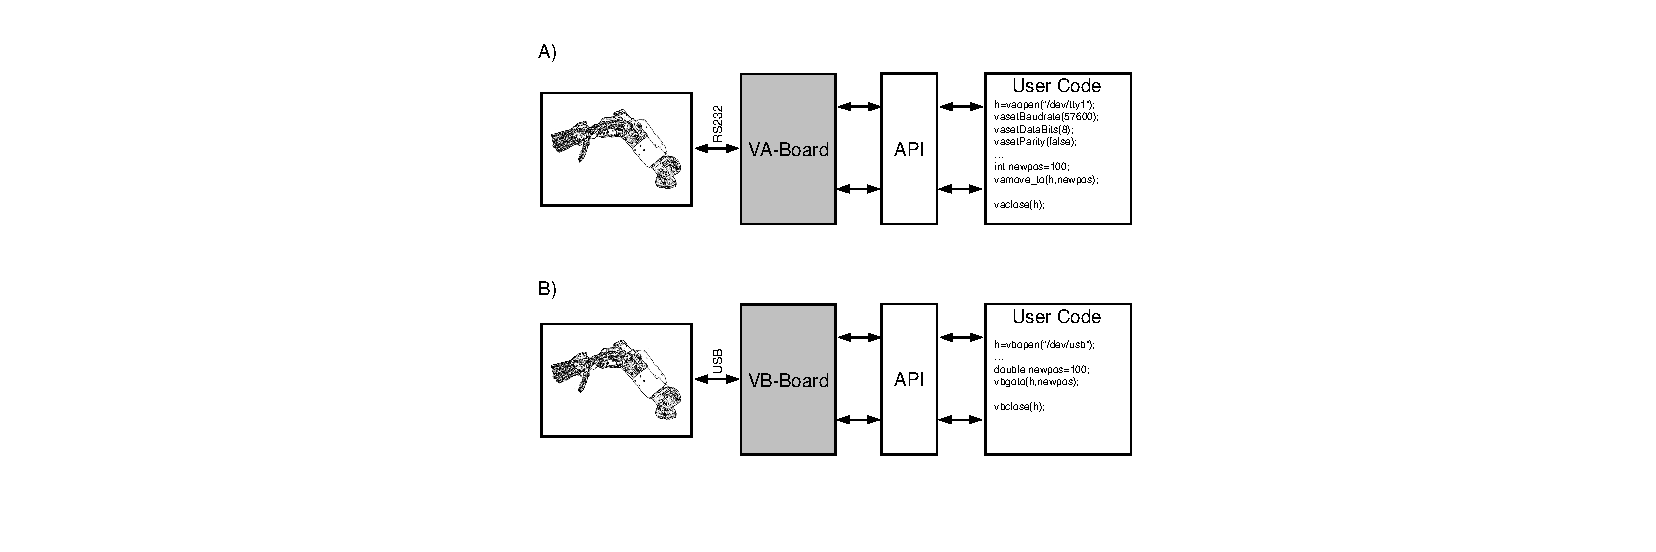
\includegraphics[width=24cm]{fig-devices1}
}
\caption{Example of code dependency. A) VABoard is a 
motor control board which interface to the robot through serial port. 
The user's code contains code to initialize the board and control the 
robot thorugh the API library provided by the vendor. B) A new 
motor control board is connected to the robot; this new device has a 
USB interface and a different API. The differences are 
are inevitably propagated to the user's code which must be 
rewritten.}\label{fig:devices1}
\end{figure}

\subsection{Device Interfaces}
An interface to a YARP device is the specification of the functionalities
it provides. In practice in C++ an interface is a virtual base class, whose 
member functions define the ensemble of  functionalities a device must 
implement in order to provide that interface.  A YARP device is a 
``wrapper'' class which implements all methods declared in its interface. 
A single device can of course expose more than a single interface 
(in C++ this is implemented through multiple
inheritance). All details specific to the hardware 
(vendor's API and library) are handled in the wrapper class and are 
hidden behind its interfaces. 
The idea is that changes in the hardware are caught by the wrapper class 
and never propagated to the user code. As a result, if interfaces are 
well designed, the impact on the code due to hardware change is minimized. 
%
Of course, unique features of a device can be exposed in a new interface,
but without much benefit over using the vendor's code directly for that
specific feature.  And any code written using that novel interface will
need to be reworked if another device is substituted.

As discussed previously, initialization parameters may introduce annoying 
dependencies in the user's code. To solve this we have defined a common 
interface to all devices (the 
\emph{DeviceDriver} interface) which normalizes how devices are initialized
and un-initialized, and, more importantly, how initialization parameters 
are passed to them. In particular this interface defines two methods:
\begin{verbatim}
  virtual bool open(yarp::os::Searchable& config)=0;
\end{verbatim}
and
\begin{verbatim}
  virtual bool close()=0;
\end{verbatim}
This \emph{open} method initializes the device. Initialization parameters 
are passed to the function as a list of key-value entries 
(a \emph{Searchable} object),
A \emph{Searchable} can contain all 
possible parameters devices might require for initialization. Initialization 
parameters for devices 
are stored in ``.ini'' files (again in the form of a list of key-value 
entries).
A process that wants to open a device reads 
the file and transfers its content into a \emph{Searchable} object. 
This class
plays a similar role in YARP as the {\em ConfigFile} class in Player/Stage,
except generalized to also
extracting parameters expressed as command line arguments, or
passed across the network, or created in a GUI, etc. -- we abstract
across all the possible sources of configuration settings.
The configuration
object is passed to the device through the \emph{open} function. 
It is worth stressing that up to now this procedure is totally device 
independent, because the parameters are just copied and not interpreted 
by the process. It is only in the implementation of the \emph{open} method 
(in the wrapper class of the device) where the \emph{Searchable} object 
is parsed to extract the parameters that will be used to inizialize the 
device.  The \emph{Searchable} object is designed so that it can
collect information about how it is used, yielding some basic
documentation about the parameters relevant to a given device.

The \emph{close} method performs all the operations required to shut down 
the device properly and release all the resources it was using. No
parameters are required by this function.

\begin{figure}[tbp]
\centerline{
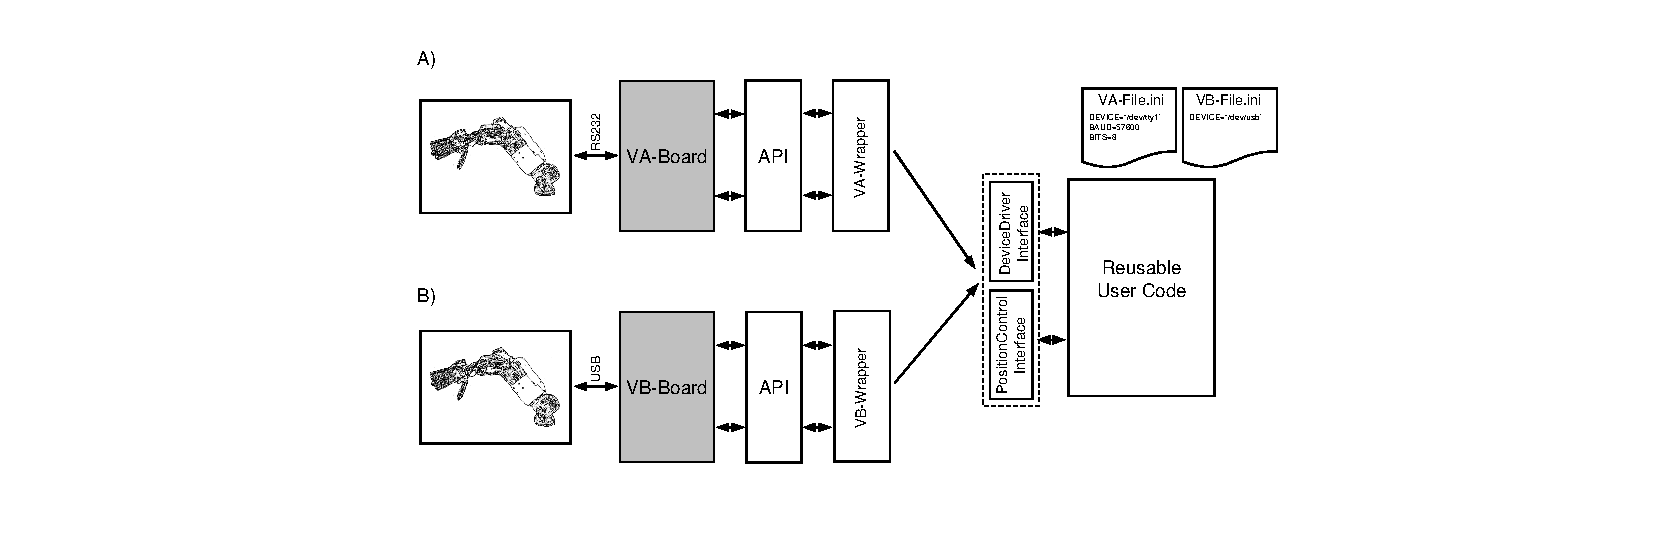
\includegraphics[width=24cm]{fig-devices2}
}
\caption{Interfaces allow code reuse. VABoard and VBBoard (see 
Figure (\ref{fig:devices1})) now implement
the same interfaces (through their respective wrapper classes). The user's 
code accesses the hardware through these interfaces and is not aware of 
the details of how the methods are actually implemented. The different 
initialization parameters are listed in configuration files and are thus 
separated. VABoard and VBBoard are now completely interchangable.}
\label{fig:devices2}
\end{figure}

YARP defines interfaces to broad families of devices. For 
example this is a partial list of the interfaces defined for generic 
devices that generate a stream of color images (frame grabbers):

\begin{itemize}

\item \emph{IFrameGrabberRgb}, methods in this interface 
provide access to the most recent frame acquired by the device, and 
information about its size (number of columns and rows);

\item \emph{IFrameGrabberControls}, specifies a set of functionalities 
to control how the device performs the acquisition, like shutter speed, 
brightness and gain.

\end{itemize}

Interfaces to motor control devices are more difficult to define. Control 
boards designed for industrial applications have often a quite stadard 
interface which provides a PID control algorithm and position or velocity 
control modes. Things become more complicated when we consider also 
programmable devices that can implement virtually an infinite type of 
functionalities and control algorithms. 
For this reason interface to control boards has been defined on the basis 
of the control paradigm they implement. Accordingly, YARP defines:

\begin{itemize}

\item \emph{IEncoder}: group all methods providing access to the motor 
encoders, like methods for reading the current position and velocity of 
each axis;

\item \emph{IPositionControl}: methods to control each axis 
by specifying its position;

\item \emph{IVelocityControl}: methods to control each axis 
by specifying its velocity;

\item \emph{ITorqueControl}: defiens methods to control the amount of 
force/torque exerted by each axis.

\end{itemize}

These last interfaces are indipendent of the particular algorithm the 
control board implements to realize the corresponding functionality. 
These details are delegated to specific interfaces. For example 
\emph{IPidControl} includes methods to interface to a PID controller, 
like for example read or set the values of the gains.

To summarize, interfaces captures similarities amoung devices and 
allows separating device dependent from user code. To the 
extent that user code uses interfaces shared by other devices, 
another device can be substituted later without change to that part. This 
includes devices with different initialization procedures, or different
APIs (see Figure (\ref{fig:devices2})).

\subsection{A factory of devices}
Forcing device access through 
interface achieve a good level of separation between vendor/device 
specific APIs and user level code. Interfaces alone, however, do not 
guarantee a complete level of separation. In practice users must still 
specify the type of device they want to create. Care must be taken to 
avoid that this introduces device dependent code. A common software 
engineering practice is to \emph{localize object creation} so to 
minimize the amount of code that is responsible for object creation 
and initialization. 
We have seen that in YARP part of this is realized by the 
\emph{DeviceDriver} interface, which forces all initialization procedures 
to be performed inside the \emph{open} method. Device creation is instead 
delegated to a \emph{factory}. The \emph{factory} contains a list of 
all devices available in YARP and the corresponding functions to call 
to create them. It receives a list of initialization parameters, 
creates the device, and initializes it 
through the \emph{DeviceDriver} interface. If the process is successfull 
a valid pointer to the device is returned. This pointer is the only 
``access point'' to the device and its interfaces. Other interfaces can 
be obtained by casting this pointer to the appropriate virtual class 
(in C++ this can be safely done through dynamic cast). 

The whole process of creation, initialization and interface access is 
managed by the \emph{PolyDriver} object. The user has only direct access 
to the \emph{PolyDriver}, to which he asks the creation of a particolar 
device, through the \emph{PolyDriver::open())} method. This request is 
forwarded to the \emph{factory} which creats an instance of the particular 
device driver the user wants to use. Device drivers are uniquely identified 
through a symbolic name; the \emph{factory} searches the list of device 
for an entry whose name matches the one that is requested and, if the match 
is found, it calls the appropriate constructor. If the driver is successfully 
created the \emph{factory} returns a valid pointer which is stored inside 
the \emph{PolyDriver}. The lifecycle of the device is managed by the 
\emph{PolyDriver}; the user can access only to copies of this pointer 
thourgh calls to the \emph{PolyDriver::view()} method, which performs 
a dynamic cast of the internal pointer to the device driver to expose 
the requested interface before returning it (this mechniam is sketched 
in Figure (\ref{fig:devices4}) \emph{NOTE: not sure this picture is 
really needed, consider removing it}).

\begin{figure}[tbp]
\centerline{
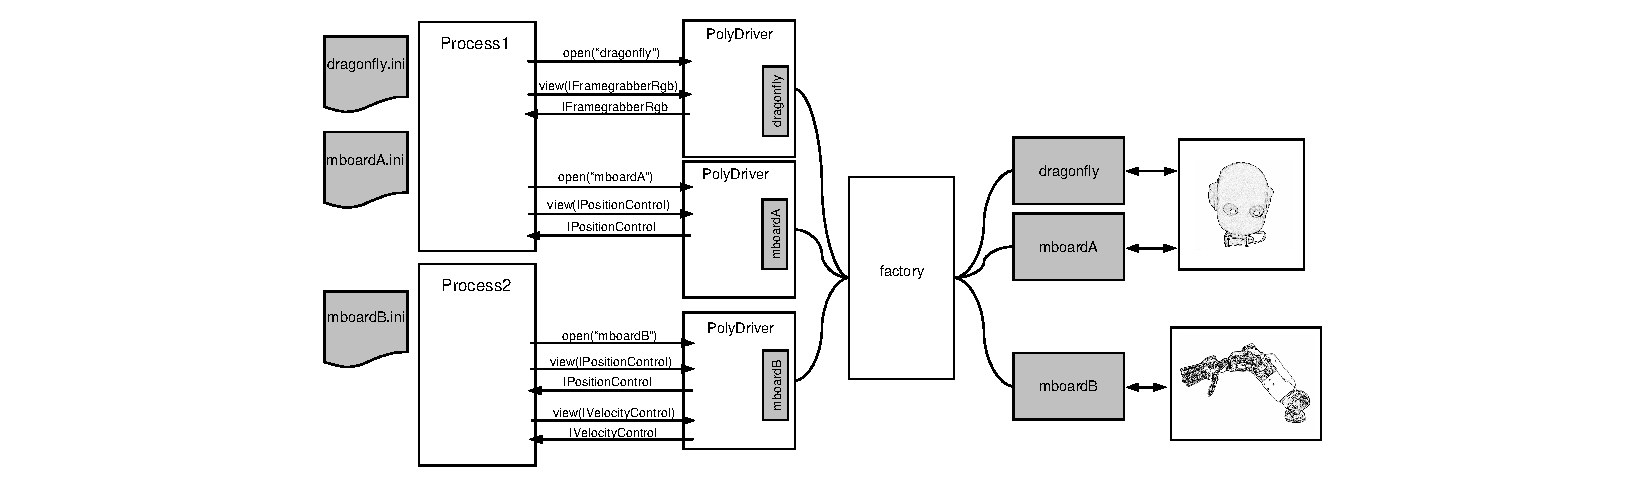
\includegraphics[width=20cm]{fig-devices4}
}
\caption{Device creation and initialization. Creation of 
devices in YARP in delegated to a \emph{factory} object. Users 
access devices through instances of the \emph{PolyDriver}. The 
Figure describes the following situation. Process1 controls a robotic
head and needs to access to the robot frame grabber (whose symbolic name 
is ``dragonfly'') and to the control board connected to the motors of 
the head (``mboardA''). Process1 creates \emph{PolyDriver} and opens 
the device; the symbolic name of the device is passed as a parameter
of the \emph{open} function, together with initialization parameters 
read from a .ini file. The \emph{PolyDriver} hands over these parameters 
to the \emph{factory} which creates an instance of the device and returns
it to the \emph{PolyDriver}. Subsequent calls to the driver are entirely 
handled by the \emph{PolyDriver} itself. Process1 calls \emph{view} to 
acquires the appropriate interfaces to the device. A similar procedure 
is performed by the same process or other processes (Process 2 in Figure) 
to create instances of different devices.}\label{fig:devices4}
\end{figure}

\subsection{An example: accessing a motor control board}
For example suppose we want to use the \emph{test\_motor} device. In 
YARP this is a fake device which simulates a control board controlling 
4 axes. This device supports the \emph{IPositionControl} and 
\emph{IVelocity} interfaces. To begin with, we first create an 
instance of the \emph{PolyDriver}. The actual device is create by 
calling the \emph{PolyDriver::open()} method specifying the symbolic 
name of the device (e.g. \emph{test\_motor}):

\begin{verbatim}
  PolyDriver device;
  device.open(\"test\_motor\");
\end{verbatim}

Now we can ask interfaces to \emph{test\_motor} by calling the 
\emph{PolyDriver::view()}method:

\begin{verbatim}
  IPositionControl *ipos=0;
  device.view(ipos);

  IVelocityControl *ivel=0;
  device.view(ivel);
\end{verbatim}

Checking if ivel and ipos are not null assures that \emph{test\_motor} 
really supports the respective interfaces.

We can now call methods of the \emph{IPositionControl} interface to control 
joint $0$ to move to the angular position of $40deg$, with the velocity 
of $5\frac{deg}{s}$ and acceleration of $100\frac{deg}{s^2}$:

\begin{verbatim}
ipos->setRefAcceleration(0, 100);
ipos->setRefSpeed(0, 5)
ipos->positionMove(0, 40);
\end{verbatim}

Or use the \emph{IVelocity} interface to servo joint 1 at the velocity 
of $5\frac{deg}{s}$ with the acceleration of $100\frac{deg}{s^2}$:

\begin{verbatim}
ivel->setRefAcceleration(1,100);
ivel->velocityMove(1, 5);
\end{verbatim}

\subsection{Device Remotization: Binary Interfaces}
A final level of separation is achieved by supporting device remotization. 
This feature is important because flexibility imposes 
that processes are written so that they can be easily moved across 
distinct machines, if needed. Knowledge of whether a process is accessing 
a given device locally or remotely would clearly limit this flexibility, 
because it would force modification in the code of the process itself. 
Remotization also facilitate portability across different platforms, as 
it naturally defines a ``binary'' interface that can 
be used to make resources available on one platform to processes compiled 
and running on a different one. This decouple the compilation, build 
environment, libraries, operating system and language dependencies of 
hardware and user software.

The remotization mechanism relies on the communication layer (see \emph{add 
reference to port section} and on two \emph{Network Wrappers} one acting 
as a \emph{Server} and the other acting as a \emph{Client}. 
Both \emph{Network Wrappers} are devices implementing the very same set 
of interfaces as the device they wrap. Both devices act proxies and talk 
to each other using a predefined protocol, which involves one or more 
YARP Ports configured for RPC or streaming (see \ref{fig:devices3})

The \emph{Server Wrapper} creates an instance of the wrapped device and 
forwards requests from the incoming connections to the device by calling 
its interfaces. If the request involves a reply this is sent back to the 
calling port so that it is received by the remote client. The mechanism 
used by the \emph{Server Wrapper} to access the local device is the same 
we have described for the user code; as 
such the \emph{Server Wrapper} is a total independent entity that can be 
reused for all devices implementing the same interface(s). 

The process at the other side of the communication creates the 
\emph{Client Wrapper}. The latter exports exactly the same interfaces as the 
device driver it wraps so the process is not aware that it is not talking to 
a real device. The job of the \emph{Client Wrapper} is to convert calls from 
the user code in packets of bytes and send them to the other end of the 
communication, and, in case a reply is expected, waits for data and dispatch 
it to the calling process. The responsibility of the proxies among the other 
things is to perform the marshalling and de-marshalling of the information 
so that it is correctly interpreted by the distinct platforms (this is 
required for systems in which data is represented with different standards).

\begin{figure}[tbp]
\centerline{
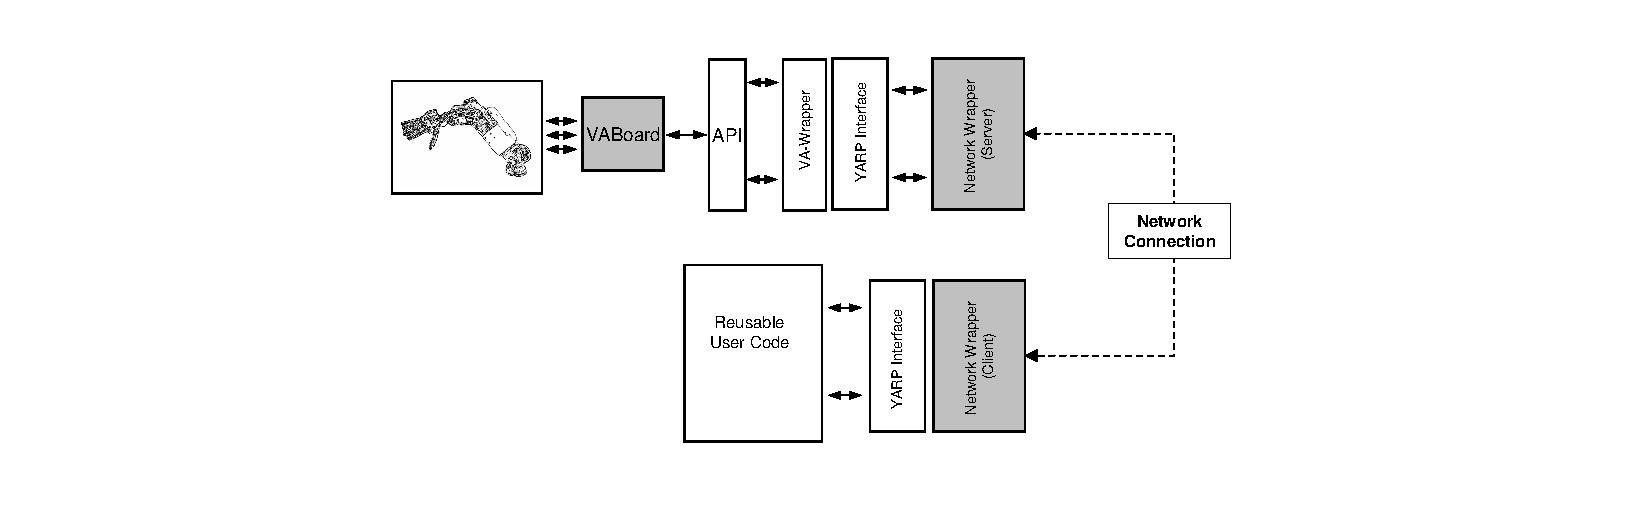
\includegraphics[width=24cm]{fig-devices3}
}
\caption{Network wrappers allow device remotization. A generic Network 
wrapper exports the YARP interfaces so that they can be accessed remotely 
by another machine through an RPC mechanism. At the other side of the 
communication the client wrapper exports the network interface back 
to the YARP interfaces from which the device is transparently accessed 
by the client code. The only difference between a local device and a 
remote one is in term of performances (the time it takes to execute 
a given function).
}\label{fig:devices3}
\end{figure}

Orphan text:

The goal of YARP is to support humanoid robotics, in which a broad 
variety of hardware is often employed. In YARP we try to facilitate code 
exchange between researchers, especially when this speeds up the time 
it takes to develop a platform and use it for research. In this sense 
device-level software development is a very time consuming and tedious 
task, so the possibility to share code in this context is extremely 
profitable. YARP devices consists in a set of \emph{wrapper classes}, 
which usually link vendor's libraries.... 

%%% SOME UNUSED TEXT moved to section-scrapyard.tex

